\documentclass[11pt,letterpaper]{article}
\usepackage[utf8]{inputenc}
\usepackage{caption} % for table captions
\usepackage{amsmath} % for multi-line equations and piecewises
\usepackage{graphicx}
%\usepackage{textcomp}
\usepackage{xspace}
\usepackage{verbatim} % for block comments
%\usepackage{subfig} % for subfigures
\usepackage{enumitem} % for a) b) c) lists
\newcommand{\Cyclus}{\textsc{Cyclus}\xspace}%
\newcommand{\Cycamore}{\textsc{Cycamore}\xspace}%
\usepackage{tabularx}
\usepackage{color}
\definecolor{bg}{rgb}{0.95,0.95,0.95}
\newcolumntype{b}{X}
\newcolumntype{f}{>{\hsize=.15\hsize}X}
\newcolumntype{s}{>{\hsize=.5\hsize}X}
\newcolumntype{m}{>{\hsize=.75\hsize}X}
\usepackage{titling}
\usepackage[hang,flushmargin]{footmisc}
\renewcommand*\footnoterule{}
\usepackage[newfloat]{minted}
\newenvironment{code}{\captionsetup{type=listing}}{}
\SetupFloatingEnvironment{listing}{name=Code}

\usepackage{tikz}


\usetikzlibrary{shapes.geometric,arrows}
\tikzstyle{process} = [rectangle, rounded corners, minimum width=1cm, minimum height=1cm,text centered, draw=black, fill=blue!30]
\tikzstyle{arrow} = [thick,->,>=stealth]


\graphicspath{{images/}}
 
\title{Numerical Experiments for Verifying Demand Driven Deployment Algorithms}
\author{Jin Whan Bae, Gwendolyn Chee, Kathryn Huff}


\begin{document}
	\maketitle
	\hrule

\section{Introduction}
For many fuel cycle simulations, it is currently up to the user to define
a deploy scheme, or facility parameters, to make sure that there's no gap
in the supply chain. Or, the same goal is achieved by setting the
\texttt{facility} capacity to infinity, which does not reflect real-world
conditions. 

The Demand-Driven Cycamore Archetype project (NEUP-FY16-10512) aims to develop \Cycamore demand-driven deployment capabilities.
The developed algorithm, in the form of \Cyclus \texttt{Institution}
agent, deploys \texttt{Facilities} to meet the front-end and back-end demands of the 
fuel cycle.

This report describes numerical tests for non-optimizing, deterministic-optimizing and stochastic-optimizing prediction algorithms.

These prediction models are being developed by the University of South Carolina. 
In this report, we discuss numerical experiments for testing the non-optimizing, 
deterministic optimizing and stochastic optimizing methods. The numerical 
experiments will be designed for both the once through nuclear fuel 
cycle and advanced fuel cycles. 

\section{Method}
This report lists necessary capabilities of the new \Cyclus \texttt{institute}
for demand-driven deployment of fuel cycle facilities. 
Then the report lists tests to check correct implementation of the capabilities,
with a sample fuel cycle with well-defined facility parameters.


\section{Configuration}
The user defines prototypes to be deployed for fuel facilities,
and reactor deployment scheme.  The reactor deployment causes the demand of fuel
which triggers fuel facility deployment. The detailed input file XML input schema
is shown in Appendix A. 

\section{Algorithm Flow}

The algorithm, upon entering, creates a supply chain with the fuel facilities and
the reactor. Then, at every timestep it calculates the expected demand from each fuel cycle
facility and makes decisions to deploy or decommission. As a reference, the time step
execution for \Cyclus is illustrated in figure \ref{diag:time}.

\begin{figure}[H]
\centering
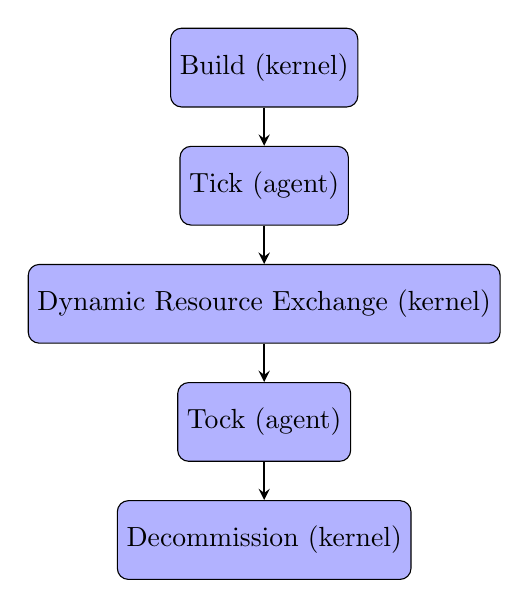
\begin{tikzpicture}[node distance=1.5cm]
\node (Build) [process] {Build (kernel)};
\node (Tick) [process, below of=Build] {Tick (agent)};
\node (DRE) [process, below of=Tick]{Dynamic Resource Exchange (kernel) };
\node (Tock) [process, below of=DRE]{Tock (agent)};
\node (Decom) [process, below of=Tock] {Decommission (kernel)};

\draw [arrow] (Build) -- (Tick); 
\draw [arrow] (Tick) -- (DRE);
\draw [arrow] (DRE) -- (Tock);
\draw [arrow] (Tock) -- (Decom);
\end{tikzpicture}
\caption{Each timestep in \Cyclus follows the five steps in order. Processes labeled
         kernel are executed by the \Cyclus framework, whereas processes labeled agent
         are executed by individual agents. What happens in the `Tick' and `Tock' is
         thus unique to each archetype.}
\label{diag:time}
\end{figure}

\subsection{Upon Entering (\texttt{Enternotify})}

The algorithm creates a supply chain with the fuel facilities,
then calculates the demand for each facility for a unit quantity of fuel
(example in figure \ref{diag:dem}). It also orders to build fuel cycle
facilities for the reactors at timestep 1.

\begin{figure}[H]
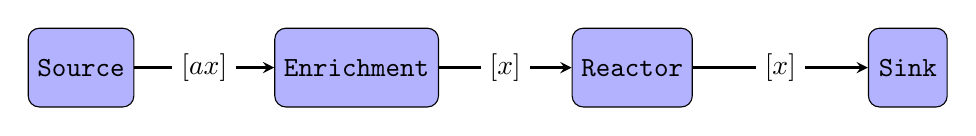
\begin{tikzpicture}[node distance=3.5cm]
\node (source) [process] {\texttt{Source}};
\node (enrichment) [process, right of=source] {\texttt{Enrichment}};
\node (reactor) [process, right of=enrichment]{\texttt{Reactor}};
\node (sink) [process, right of=reactor]{\texttt{Sink}};

\draw [arrow] (source) -- (enrichment) node[midway,fill=white] {$[ax]$}; 
\draw [arrow] (enrichment) -- (reactor) node[midway,fill=white] {$[x]$}; 
\draw [arrow] (reactor) -- (sink) node[midway,fill=white] {$[x]$}; 
\end{tikzpicture}
\caption{Simple demand flow of materials. The values in the bracket are demands calculated
         by the algorithm. The \texttt{Reactor} demands $x$ amount of fuel,
         which translates into demands of $x$ from \texttt{Enrichment} and \texttt{Sink}.
         The \texttt{Source} has a demand of $a x$ to take in for enrichment losses.
         $a \approx 9 $ for 3\% enrichment.}
\label{diag:dem}
\end{figure}

\subsection{Tick}
The algorithm calculates the fuel demand
from the fleet of reactors at one timestep ahead, and the corresponding demand for fuel facilities.
The current capacity of each fuel cycle facility is also calculated. If the capacity
is smaller than the demand, the algorithm orders to build more facilities to meet the demand,
so that the fuel demand is met for the next timestep.

\section{Simulation parameter for Test Scenarios}
Simple parameters are given to fuel cycle facilities for the numerical testing of 
the algorithm.  

Table \ref{tab:testscenario} provides basic parameters for each test scenario. Table \ref{tab:reactor} provides the parameters for the \texttt{source} and \texttt{reactors} in the test scenarios.

\begin{table}[h]
	\centering
	\begin{tabularx}{\textwidth}{bsb}
		\hline
		Test Scenario Parameters & Value & Units \\
		\hline
		Duration & 3 & timesteps \\
		Timestep & 1 & month \\
		Start Month & 1 & month \\
		Start Year & 2000 & year \\
		\hline
	\end{tabularx}
	\caption {Basic Test Parameters}
	\label{tab:testscenario}
\end{table}

\begin{table}[h]
    \centering
    \begin{tabularx}{\textwidth}{bbb}
       \hline
       Source Parameters & Value & Units \\
       \hline
       Throughput & 1 & kg \\
       Output Commodity & fresh uox & \\
       \hline
       Reactor Parameters & Value & Units \\
       \hline
       Cycle Time & 1 & timesteps \\
       Refuel Time & 0 & timesteps \\
       Lifetime & 1 & timesteps \\
       Power Capacity & 1& MWe \\
       Assembly Size & 1 & kg \\
       \# assemblies per core & 1 & \\
       \# assemblies per batch & 1 & \\
       Input Commodity & fresh uox & \\
       Input Commodity & spent uox & \\
       \hline
    \end{tabularx}
    \caption {Reactor Parameters}
    \label{tab:reactor}
\end{table}

\begin{comment}
Should i add a table with the recipes for fresh and spent uox? Seems unnecessary since its not explicitly used in any analytical solutions.
\end{comment}

\pagebreak

\section{Numerical Tests for the Non-optimizing prediction method}
To ensure that the non-optimizing prediction model is working correctly, a variation of input files that uses the non-optimizing method archetype to deploy or decommission facilities is tested to determine if their outputs match the analytical solution. In this section, the tests that must be met is described based on the parameters defined in table \ref{tab:testscenario} and \ref{tab:reactor} and analytical solution of a defined simple scenario. Unit test examples are included in Appendix B.

The tests are split into test A types and test B types. Test A refers to the test scenarios where facilities are expected to be deployed. Test B refers to the test scenarios where facilities are expected to be decommissioned. 

The aim with the various test scenarios are to check if the non-optimizing method archetype will deploy or decommission facilities correctly when there is a variation in the three possible input functionalities.  
\begin{enumerate}
	\item There is an initial demand. 
	\item There is an initial facility already present. 
	\item There is a growth in the demand.
\end{enumerate}

The functionalities are tested alone, and also mixed and matched to give various test scenarios to determine if the non-optimizing method archetype will deploy or decommission facilities correctly in the presence of more than one functionality. For ease of determining the analytical solution, each functionality is standardized in the test scenarios. This means that the three input functionalities are restricted to be:  

\begin{enumerate}
	\item There is an initial demand of 1 unit. 
	\item There is 1 initial facility already present. 
	\item There is a growth rate of 1 (100\%) for the demanded resource.
\end{enumerate}



\subsection{Test A-1: There is an initial demand for 1kg of fuel.}

\begin{comment}
To ensure that the non-optimizing prediction model is working correctly, each function of the code must be tested to determine if its output matches the analytical solution for the specified test scenario. In this section, the tests that must be met is described based on the parameters defined in table \ref{tab:reactor} and \ref{tab:everythingelse} and analytical solution of a defined simple scenario. Unit test examples are included in Appendix B.
\end{comment}

\noindent
\textbf{Test 1: A reactor outputs the user defined power capacity when deployed and does not output
power capacity when decommissioned.} \\
Test Scenario: A single reactor is deployed at time step 2 and decommissioned at time step 4. There is an infinite source of fuel for the reactor. \\
Analytical Solution: During cycle time, the reactor will have a power output of 1000MWe. Therefore,
there is only be power output of 1000MWe at time steps 2 and 3. The analytical solution of
the power output of the reactor per time step is given in table \ref{tab:test-power}.

\begin{table}[H]
     \centering
    \begin{tabularx}{\textwidth}{bbb}
       \hline
       Timestep & Reactor Power Output (MWe) \\
       \hline
       1 & 0 \\
       2 & 1000 \\
       3 & 1000 \\
       4 & 0 \\
       \hline
    \end{tabularx}
    \caption {Analytical solution of the power output of the reactor per time step}
    \label{tab:test-power}
\end{table}

\noindent
\textbf{Test 2: A reactor outputs the user defined power capacity during its cycle time and not during its refuel time.} \\
Test Scenario: A single reactor is deployed at time step 2 and decommissioned at time step 87 \\
Analytical Solution: Based on the reactor parameters defined in table 1, the reactor will have a cycle time of 2 time steps and a refuel time of 1 time step. Therefore, there is only be power output of 1000MWe during cycle time steps. The analytical solution of the power output of the reactor per time step is given in table \ref{tab:test-cycles}.

\begin{table}[H]
     \centering
    \begin{tabularx}{\textwidth}{bbb}
       \hline
       Timestep & Reactor Power Output (MWe) \\
       \hline
       1 & 0 \\
       2 & 1000 \\
       3 & 1000 \\
       4 & 0 \\
       5 & 1000 \\
       6 & 1000 \\
       7 & 0 \\
       8 & 0 \\
       \hline
    \end{tabularx}
    \caption {Analytical solution of the power output of the reactor per time step}
    \label{tab:test-cycles}
\end{table}

\noindent
\textbf{Test 3: A facility that produces reactor’s input commodity (fuel) is deployed when the amount of fuel available is below the amount of fuel required by the reactor.} \\
Test Scenario: A single reactor is deployed at time step 2.\\
Analytical Solution: Based on the simple supply chain example in figure \ref{diag:dem} and enrichment facility parameters defined in table \ref{tab:everythingelse}, an enrichment facility must be deployed at time step 2 to meet fuel demand. The analytical solution of the enrichment facility deployment per time step is given in table \ref{tab:test-fuel}.

\begin{table}[H]
     \centering
    \begin{tabularx}{\textwidth}{bbb}
       \hline
       Timestep & Enrichment Facility deployment  \\
       \hline
       1 & 0 \\
       2 & 1 \\
       3 & 0\\
       \hline
    \end{tabularx}
    \caption {Analytical solution of the number of fuel facilities deployed per time step}
    \label{tab:test-fuel}
\end{table}

\noindent
\textbf{Test 4: An appropriate number of facilities that produces reactor's input commodity (fuel) is deployed to meet the demand of the amount of fuel required by the reactor, when the initial fuel supply is non-zero.} \\
Test Scenario: An initial fuel supply of 100kg. 2 reactors deployed at time step 2. \\
Analytical solution: Based on table \ref{tab:reactor}, each reactor has a fuel demand of 300kg per time step. Therefore, the fuel supply is 100kg at time step 1 and is 700kg at time steps 2 and 3. The analytical solution of fuel quantity per time step is given in table \ref{tab:test-fueldemand}  

\begin{table}[H]
     \centering
    \begin{tabularx}{\textwidth}{bbb}
       \hline
       Timestep & Fuel Quantity (kg)  \\
       \hline
       1 & 100 \\
       2 & 700 \\
       3 & 700\\
       \hline
    \end{tabularx}
    \caption {Analytical solution of the fuel available per time step}
    \label{tab:test-fueldemand}
\end{table}

\noindent
\textbf{Test 5: The fuel supply is within plus-minus the output of 1 fuel-producing facility of the reactor demand for fuel for all time steps.} \\
Test Scenario: A reactor is deployed at timesteps 2, 3 and 4.\\
Analytical Solution: Based on table \ref{tab:reactor}, each reactor has a fuel demand of 300kg per time step. If an appropriate number of enrichment facilities is deployed to meet fuel demand, the difference between fuel quantity and fuel demand will be 100kg per time step. The analytical solution of difference between fuel quantity and fuel demand per time step is given in table \ref{tab:test-fueldiff}.  

\begin{table}[H]
     \centering
    \begin{tabularx}{\textwidth}{bbbb}
       \hline
       Timestep & Fuel Quantity (kg) & Fuel Demand (kg) & Difference (kg)\\
       \hline
       1 & 100 & 0 &100\\
       2 & 400 & 300 &100\\
       3 & 700 & 600 &100\\
       4 & 1000 & 900 &100\\
       \hline
    \end{tabularx}
    \caption {Analytical solution of the difference between fuel quantity and fuel demand per time step}
    \label{tab:test-fueldiff}
\end{table}

\noindent
\textbf{Test 6: A fuel-producing facility is decommissioned when the amount of fuel available exceeds the the amount of fuel required by the reactor by 1 fuel-producing facility's fuel output for the number of user-defined consecutive time steps.} \\
Test Scenario: An enrichment facility is deployed at time step 2. \\
Analytical Solution: Based on table \ref{tab:everythingelse}, the supply of fuel must exceed demand by 1 enrichment facility output for 3 consecutive time steps before it is decommissioned. Therefore, the enrichment facility must be decommissioned at time step 5. The analytical solution of the enrichment facility deployment per time step is given in table \ref{tab:test-supplymoredemand}. 

\begin{table}[H]
     \centering
    \begin{tabularx}{\textwidth}{bbb}
       \hline
       Timestep & Enrichment Facility deployment \\
       \hline
       1 & 0 \\
       2 & 1 \\
       3 & 1 \\
       4 & 1 \\
       5 & 0 \\
       \hline
    \end{tabularx}
    \caption {Analytical solution of the number of fuel facilities deployed per time step}
    \label{tab:test-supplymoredemand}
\end{table}

\noindent
\textbf{Test 7: A facility that produces fuel producing facility's input commodity is deployed when the amount of input commodity is below the amount required by the fuel producing facility}. \\
Test Scenario: An enrichment facility is deployed at time step 2. \\
Analytical Solution: Based on the simple supply chain example in
figure \ref{diag:dem}, a source facility must be deployed at time step 2 to meet natural uranium demand. The analytical solution of the source facility deployment per time step is given in table \ref{tab:test-NUdemand}. 

\begin{table}[H]
     \centering
    \begin{tabularx}{\textwidth}{bbb}
       \hline
       Timestep & Source Facility deployment  \\
       \hline
       1 & 0 \\
       2 & 1 \\
       3 & 0 \\
       \hline
    \end{tabularx}
    \caption {Analytical solution of the number of source facilities deployed per time step}
    \label{tab:test-NUdemand}
\end{table}

\noindent
\textbf{Test 8: An appropriate number of facilities that produces fuel-producing facility's input commodity is deployed to meet the demand of input commodity required by the fuel producing facility, when the initial input commodity is non-zero.} \\
Test Scenario: An initial natural uranium supply of 1000kg. 1 enrichment facility deployed at time step 2. \\
Analytical solution: Based on table \ref{tab:everythingelse}, each enrichment facility has a SWU capacity of 2000 SWU per time step and each source facility has a throughput of 3000kg per time step. Based on table \ref{tab:simulationparameters}, approximately 3500kg of natural uranium is required for enrichment SWU capacity of 2000. Therefore, 1 source facility must be commissioned to meet the demand of one enrichment facility. Therefore, the natural uranium supply is 1000kg at time step 1 and is 4500kg at time steps 2 and 3. The analytical solution of fuel quantity per time step is given in table \ref{tab:test-NUdemand2}.  

\begin{table}[H]
     \centering
    \begin{tabularx}{\textwidth}{bbb}
       \hline
       Timestep & Natural Uranium Quantity (kg)  \\
       \hline
       1 & 1000 \\
       2 & 4500 \\
       3 & 4500\\
       \hline
    \end{tabularx}
    \caption {Analytical solution of the fuel available per time step}
    \label{tab:test-NUdemand2}
\end{table}

\noindent
\textbf{Test 9: The supply of input commodity for the fuel-producing facility is within plus-minus the output of 1 facility that produces it, of the fuel-producing facility's demand for the input commodity for all time steps.} \\
Test Scenario: An enrichment facility is deployed at timesteps 2, 3 and 4.\\
Analytical Solution: Based on table \ref{tab:simulationparameters}, each enrichment facility has a natural uranium demand of 3412kg per time step. If an appropriate number of source facilities is deployed to meet natural uranium demand, the difference between fuel quantity and fuel demand will be 88kg per time step. The analytical solution of difference between natural uranium quantity and natural uranium demand per time step is given in table \ref{tab:test-NUdiff}.  

\begin{table}[H]
     \centering
    \begin{tabularx}{\textwidth}{bbbb}
       \hline
       Timestep & Natural Uranium Quantity (kg) & Natural Uranium Demand (kg) & Difference (kg)\\
       \hline
       1 & 0 & 0 & 0\\
       2 & 3500 & 3412 & 88\\
       3 &  7000 & 6824 & 176\\
       4 & 10500 & 10236 & 264\\
       \hline
    \end{tabularx}
    \caption {Analytical solution of the difference between natural uranium  quantity and natural uranium demand per time step}
    \label{tab:test-NUdiff}
\end{table}

\noindent
\textbf{Test 10: A facility that produces fuel-producing facility's input commodity is decommissioned when the amount of input commodity available exceeds the the amount of input commodity required by the fuel-producing facility by 1 facility's output for the number of user-defined consecutive time steps.} \\
Test Scenario: A source facility is deployed at time step 2. \\
Analytical Solution: Based on table \ref{tab:everythingelse}, the supply of natural uranium must exceed demand by 1 source facility output for 3 consecutive time steps before it is decommissioned. Therefore, the source facility must be decommissioned at time step 5. The analytical solution of the source facility deployment per time step is given in table \ref{tab:test-supplymoredemand2}. 

\begin{table}[H]
     \centering
    \begin{tabularx}{\textwidth}{bbb}
       \hline
       Timestep & Source Facility deployment \\
       \hline
       1 & 0 \\
       2 & 1 \\
       3 & 1 \\
       4 & 1 \\
       5 & 0 \\
       \hline
    \end{tabularx}
    \caption {Analytical solution of the number of source facilities deployed per time step}
    \label{tab:test-supplymoredemand2}
\end{table}


\begin{comment}
commented out till further time
\subsection{Deterministic-Optimizing/Stochastic prediction method}
The following conditions need to be satisfied for each segment of the fuel cycle. 

\begin{enumerate}
\item Do all the \texttt{Reactor}s run? 
\begin{minted}{c++}
TEST(ReactorTests, DDDeploy_DO) {
    [Example input with the following attributes:]
        [int simdur = 20;]
        [Defines reactor with zero refueling cycle and operation 
        cycle of 1 month]
        [Defines fuel cycle facilities parameters]
        [Defines Reactor Deploy Scheme / Power Demand]
        [Increasing Fuel Demand with Time]
    [Run test]
    [Test if Reactor has no zero values in output Timeseriespower]
}
\end{minted}
\item  Do all the \texttt{Reactor}s run at full capacity (not lacking fuel)? 
\begin{minted}{c++}
TEST(ReactorTests, DDDeploy_DO) {
    [Example input with the following attributes:]
        [int simdur = 20;]
        [Defines reactor with zero refueling cycle, power capacity 
        of x and operation cycle of 1 month]
        [Defines fuel cycle facilities parameters]
        [Defines Reactor Deploy Scheme / Power Demand]
        [Increasing Fuel Demand with Time]
    [Run test]
    [Test if Reactor has x value in output Timeseriespower]
}
\end{minted}

\item Is the objective function optimized?

\item Is the constraint followed? 

\item  Do the related fuel cycle facilities get deployed upon demand?
\begin{minted}{xml}
TEST(ReactorTests, DDDeploy_NO) {
    [Example input with the following attributes:]
        [int simdur = 20;]
        [Defines reactor with zero refueling cycle and operation 
        cycle of 1 month]
        [Defines fuel cycle facilities parameters]
        [Defines Reactor Deploy Scheme / Power Demand]
        [Increasing Fuel Demand with Time]
    [Run test]
    [Test if fuel facility is deployed in the beginning]
    [Test if fuel facility is deployed later in the simulation 
    (have analytic solution)]
}
\end{minted}

\item Do the related fuel cycle facilities exit upon demand decrease?
\begin{minted}{xml}
TEST(ReactorTests, DDDeploy_NO) {
    [Example input with the following attributes:]
        [int simdur = 20;]
        [Defines reactor with zero refueling cycle and operation 
        cycle of 1 month]
        [Defines fuel cycle facilities parameters]
        [Defines Reactor Deploy Scheme / Power Demand]
        [Decreasing Fuel Demand with Time]
    [Run test]
    [Test if fuel facility is deployed in the beginning]
    [Test if fuel facility exits later in the simulation (have 
    analytic solution)]
}
\end{minted}


\end{enumerate}



\section{Advanced Fuel Cycles}
\end{comment}

\section{Appendix A - parameter configuration}

First, the user defines the prototypes to be deployed
to support the reactor.

\begin{code}

\begin{minted}[bgcolor=bg]{xml}
<interleave>
  <element name="institution">
    <data type="string"/>
  </element>
    <element name="prototypes">
      <oneOrMore>
        <element name="val">
          <data type="string"/>
        </element>
      <oneOrMore>
    </element>
</interleave>

\end{minted}
\captionof{listing}{Fuel cycle facility prototype definition}
\label{code:pro}
\end{code}


Then deployment of the power-producing reactors is defined, and the user
is given two choices:
\begin{itemize}
  \item Manually define the deployment scheme of reactors (code \ref{code:man_reac})
  \item Define power demand equation (code \ref{code:fun_reac})
\end{itemize}

\begin{code}
\begin{minted}[bgcolor=bg]{xml}
<interleave>
  <element name="reactors">
    <oneOrMore>
      <element name="val">
        <data type="string"/>
      </element>
    </oneOrMore>
  </element>
  <element name="build_times">
    <oneOrMore>
      <element name="val">
        <data type="int"/>
      </element>
    </oneOrMore>
  </element>
  <element name="n_build">
    <oneOrMore>
      <element name="val">
        <data type="int"/>
      </element>
    </oneOrMore>
  </element>
  <optional>
    <element name="lifetimes">
      <oneOrMore>
        <element name="val">
          <data type="int"/>
        </element>
      </oneOrMore>
    </element>
  </optional>
</interleave>
\end{minted}
\captionof{listing}{Manual definition of reactor deployment}
\label{code:man_reac}
\end{code}

\begin{code}

\begin{minted}[bgcolor=bg]{xml}
<interleave>
  <element name="growth">
    <oneOrMore>
      <element name="item">
        <interleave>
          <element name="reactors">
            <data type="string"/>
          </element>
          <element name="piecewise_function">
            <oneOrMore>
              <element name="piece">
                <interleave>
                  <element name="start">
                    <data type="int"/>
                  </element>
                  <element name="function">
                    <interleave>
                      <element name="type">
                        <data type="string"/>
                      </element>
                      <element name="params">
                        <data type="string"/>
                      </element>
                    </interleave>
                  </element>
                </interleave>
              </element>
            </oneOrMore>
          </element>
        </interleave>
      </element>
    </oneOrMore>
  </element>
</interleave>
\end{minted}
\captionof{listing}{Definition of power demand function}
\label{code:fun_reac}
\end{code}

\begin{comment}
\section{Appendix B - Sample Test Code }
\subsection{Reactor}
\noindent
\textbf{Condition 1: All the reactors run at full capacity} 
\begin{minted}{C++}
TEtST(ReactorTests, FullCapacity) {
   std::string config = 
     "  <fuel_inrecipes>  <val>fresh_uox</val>  </fuel_inrecipes>  "
     "  <fuel_outrecipes> <val>spent_uox</val>  </fuel_outrecipes>  "
     "  <fuel_incommods>  <val>uox</val> </fuel_incommods>  "
     "  <fuel_outcommods> <val>spent_uox</val>      </fuel_outcommods>  "
     "  <fuel_prefs>      <val>1.0</val>        </fuel_prefs>  "
     ""
     "  <cycle_time>2</cycle_time>  "
     "  <refuel_time>1</refuel_time>  "
     "  <assem_size>100</assem_size>  "
     "  <n_assem_core>3</n_assem_core>  "
     "  <n_assem_batch>1</n_assem_batch>  ";

  int simdur = 10 
  cyclus::MockSim sim(cyclus::AgentSpec(":cycamore:Reactor"),config
  ,simdur); 
  sim.AddSource("uox").Finalize();
  sim.AddRecipe("fresh_uox",c_uox());
  sim.AddRecipe("spent_uox".c_spentuox());
  int id. = sim.Run();

  int both_on = 2; 
  std::vector<Cond> conds; 
  conds.push_back(Cond("Value", "==",2000));
  QueryResult qr = sim.db().Query("TimeSeriesPower", &conds);
  EXPECT_EQ(both_on,qr.rows.size());  
  
  int one_on = 6; 
  std::vector<Cond> conds; 
  conds.push_back(Cond("Value", "==",1000));
  QueryResult qr = sim.db().Query("TimeSeriesPower", &conds);
  EXPECT_EQ(one_on,qr.rows.size());  

  int none_on = 2; 
  std::vector<Cond> conds; 
  conds.push_back(Cond("Value", "==",0));
  QueryResult qr = sim.db().Query("TimeSeriesPower", &conds);
  EXPECT_EQ(one_on,qr.rows.size());  
  }
\end{minted}

\noindent
\textbf{Condition 2: A new \texttt{Reactor} is deployed when the energy demand exceeds the energy produced by the current \texttt{Reactor}s?} 
\begin{minted}{C++}
TEST(ReactorTests, DeployNew) {
   std::string config = 
     "  <fuel_inrecipes>  <val>fresh_uox</val>  </fuel_inrecipes>  "
     "  <fuel_outrecipes> <val>spent_uox</val>  </fuel_outrecipes>  "
     "  <fuel_incommods>  <val>uox</val> </fuel_incommods>  "
     "  <fuel_outcommods> <val>spent_uox</val>      </fuel_outcommods>  "
     "  <fuel_prefs>      <val>1.0</val>        </fuel_prefs>  "
     ""
     "  <cycle_time>2</cycle_time>  "
     "  <refuel_time>1</refuel_time>  "
     "  <assem_size>100</assem_size>  "
     "  <n_assem_core>3</n_assem_core>  "
     "  <n_assem_batch>1</n_assem_batch>  ";

  int simdur = 10 
  cyclus::MockSim sim(cyclus::AgentSpec(":cycamore:Reactor"),config,
  simdur); 
  sim.AddSource("uox").Finalize();
  sim.AddRecipe("fresh_uox",c_uox());
  sim.AddRecipe("spent_uox".c_spentuox());
  int id. = sim.Run();
  
  int reactors_deployed = 2; 
  std::vector<Cond> conds; 
  conds.push_back(Cond("String", "==",:cycamore:Reactor)); 
  QueryResult qr = sim.db().Query("AgentEntry", &conds);
  EXPECT_EQ(reactors_deployed,qr.rows.size());
  }
\end{minted}
\end{comment}
\end{document}



